\chapter[Conception and Implementation of a Reliable Web Service with CouchDB]{Conception and Implementation of a\\Reliable Web Service with CouchDB}

\begin{quote}
{\itshape
Each node in a system should be able to make decisions purely based on local state. If you need to do something under high load with failures occurring and you need to reach agreement, you're lost. If you're concerned about scalability, any algorithm that forces you to run agreement will eventually become your bottleneck. Take that as a given.
}

\hspace{1em}---Werner Vogels, Amazon CTO and Vice President \cite[p.~13]{ASL10}\\
\end{quote}

\noindent
In chapter two, principles and concepts that generally apply to distributed systems have been explained. Principles and concepts that characterize CouchDB and make it especially well suited for the creation of reliable web services are presented in chapter three.

The goal of this chapter is to show how the principles and concepts CouchDB has been built upon, play nicely together, and almost predetermine how a reliable web service based on CouchDB ought to be implemented.

With regard to web services, the notion of reliability is defined as the ability to guarantee consistency, availability, and fault tolerance. In order to be able to maintain these guarantees, the concept of scalability (see section \ref{Scalability}) has to be included in the definition of web service reliability as well, in case that some aspects of a web service's application domain may scale to a larger size.


\section{Problem Analysis}
\label{Problem Analysis}

\paragraph{Research Method}
\begin{itemize}
	\item Identification and scope of the problem
	\item Critical literature review
	\item Establishment of the required terms and definitions
	\item Development of a model for reasoning, communicating, characterizing and predicting a CouchDB cluster's behavior
	\item Model implementation
	\item Model evaluation
\end{itemize}

\paragraph{Problem Statement}
As already mentioned in section \ref{Motivation: Consistent CouchDB Clusters}, this work's motivation is to develop a technique that allows for the creation of reliable CouchDB clusters that selectively guarantee eventual or atomic consistency of data.

The objective is a web service that provides clients with the abstraction of a single reliable CouchDB device, using a collection of possibly unreliable CouchDB units. Therefore, a scalable solution for CouchDB clusters that cannot only guarantee data consistency, but also availability and tolerance to several patterns of failure (e.g.\ crashes or network partitioning), shall be presented.

\paragraph{Scope of the Problem}
The relation between a reliable CouchDB web service and a CouchDB cluster is that a reliable CouchDB web service consists of a CouchDB cluster. The fact that a CouchDB cluster consists of several CouchDB devices, and, in turn, a CouchDB cluster is the abstraction of a single CouchDB device, means that clusters are composable, i.e.\ a CouchDB cluster can consist of several CouchDB clusters.

Hence, the problem of creating a reliable web service based on CouchDB can be reduced to the problem of creating a reliable CouchDB cluster, using data partitioning techniques as needed.

As already mentioned in section \ref{Background}, a solution for data partitioning exists with CouchDB Lounge. Because CouchDB Lounge is already documented elsewhere (see \cite{Lou10a} and \cite[p.~165]{ASL10}), there will be no further description at this point, as that would exceed the scope of this work.

\paragraph{Requirements}
\label{Requirements}
\noindent
{\bf Features and Functionalities.}
Figure \ref{mindmap_couchdb_cluster} shows features and functionalities (including their interrelation) that are needed to implement a reliable CouchDB cluster. Many of those are already part of CouchDB, or are part of existing standard architectural elements, i.e., components and connectors commonly used for providing web services. For instance, as described in the example from section \ref{Data Partitioning, Load Balancing, Clustering}, load balancing (including failover, but excluding health monitoring) can be handled by already existing connectors, namely DNS resolver and client.

The key feature to be implemented for CouchDB clusters has not been touched in previous work, at least not within that context, and was this work's initial motivation. It is the ability to choose between different consistency guarantees on a per-request basis. More precisely, it is desirable to be able to select the consistency guarantee that applies for a read/write operation when issuing the particular request.

A functionality that cannot be implemented in a generic way, is instance management. Its implementation would require knowledge of the actual hardware and software infrastructure the particular web service is deployed into. Therefore, it will not be discussed in this work.\\

\noindent
{\bf Architectural Requirements.}
Because reliability can only be achieved by avoiding single points of failure, the first architectural requirement is that of decentrality. For the sake of fault tolerance and availability, the architectural design must allow the usage of redundant instances of a component or connector, so that each instance is able to serve its purpose independently of the others.

The second architectural requirement is that components and connectors must conform to the REST constraints. As CouchDB follows the REST principles, it is advisable not to break the present architectural style when building on top of it. Accordingly, exceptions to that rule are allowed for the few cases where CouchDB itself is not RESTful.

\begin{figure}
	\begin{tikzpicture}
    \path[mindmap, concept color=red,text=black]
    node[concept] {CouchDB Cluster}[clockwise from=0]
    child[concept color=black!25!green] {
        node[concept] (res) {Crash Resilience}
        child[concept] { node[concept] {Instance Management} }
        child[concept] {
            node[concept] {Gossip Protocol}[clockwise from=-60]
                child[concept] { node[concept] {Notifica\-tion of Changed Configuration} }
                child[concept] { node[concept] {Notifica\-tion of Missed Updates} }
        }
    }
    child[concept color=blue!50] {
        node[concept] (loa) {Load Balancing}[clockwise from=-60]
        child[concept] { node[concept] (fai) {Health Monitoring} }
        child[concept] { node[concept] (fai) {Failover} }
    }
    child[concept color=green!50!blue] {
        node[concept] (rel) {Reliability}[clockwise from=-60]
        child[concept] { node[concept] {Consis\-tency} }
        child[concept] { node[concept] {Avail\-ability} }
        child[concept] { node[concept] {Fault Tolerance} }
    }
    child[concept color=violet!50] { 
        node[concept] (no) {No Single Point of Failure}[clockwise from=-120]
        child[concept] { node[concept] {Decentra\-lization} }
        child[concept] { node[concept] {Redun\-dancy} }
    }
    child[concept color=orange] {
        node[concept] (mvc) {MVCC}[clockwise from=180]
        child[concept] { node[concept] {Atomic Consistency}[clockwise from=180]
            child[concept] { node[concept] {Quorum-based Voting} }
        }
        child[concept] { node[concept] {Eventual Consistency} }
    }
    child[concept color=gray] {
        node[concept] (per) {Peer-to-Peer Replication}[clockwise from=60]
        child[concept] { node[concept] {Conflict Management} }
    };
    \begin{pgfonlayer}{background}
        \draw[circle connection bar switch color=from (white) to (black)]
            (per) edge (mvc);
        \draw[circle connection bar switch color=from (black) to (white)]
            (per) edge (res);
        \draw[circle connection bar switch color=from (white) to (black)]
            (rel) edge (res) edge (loa) edge (no) edge (mvc);
        \draw[<-, line width=6pt]
            (per) edge (mvc);
        \draw[->, line width=6pt]
            (per) edge (res);
        \draw[<-, line width=6pt]
            (rel) edge (res) edge (loa) edge (no) edge (mvc);
    \end{pgfonlayer}
\end{tikzpicture}

	\caption{Required Features and Functionalities of a Reliable CouchDB Cluster}
	\label{mindmap_couchdb_cluster}
\end{figure}


\section{System Model and Architecture}

\paragraph{System Model}
\label{System Model}
\begin{figure}
    \centering
	{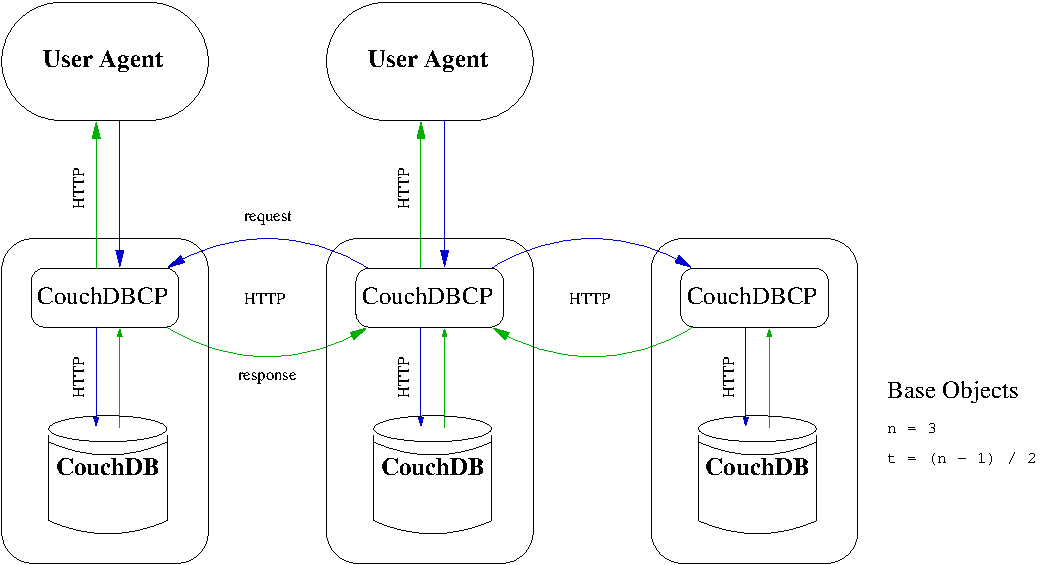
\includegraphics[width=\textwidth]{figures/system_components}}
    \caption{System Components}
    \label{system_model}
\end{figure}

Figure \ref{system_model} illustrates an example of a CouchDB cluster consisting of three identical (except for network configuration) base objects. Essentially, a base object consists of a CouchDB that is assigned to a \emph{CouchDBCP}\footnote{{\bf CouchDBCP} is an acronym for {\bf CouchDB} {\bf C}lustering {\bf P}roxy.}. A CouchDBCP is used as a gateway (more precisely as a reverse HTTP proxy) in front of a CouchDB. The two components are intended to be located nearby, connected with a high speed, low-latency network link; if not just simply located on the same computer. Client requests can be distributed across the base objects using load balancing techniques, like e.g.\ the one described in section \ref{Data Partitioning, Load Balancing, Clustering}. The CouchDBCP that receives a particular client request is referred to as the \emph{leader}.

In the example, there are two clients, each performing a data operation at the same time. The arrows indicate the HTTP requests and responses caused by the clients. The second client (from the left) has issued the request indicating that it needs to be served with atomic consistency guaranteed. The first client does not give such an indication, so that only eventual consistency semantics will be provided.\\

\noindent
{\bf Processes and Messages.}
The system's units that are able to perform computations are abstracted through the notion of \emph{process}, according to \cite[p.~26]{GR06}. The system is composed of a set of uniquely identified processes that know of each other, and run the same local algorithm. The sum of these copies comprises the actual distributed algorithm.

The processes communicate by exchanging uniquely identified messages, which are exchanged through communication \emph{links}.

For a more comprehensive and universal description of distributed computation abstractions, like processes and links, among other things, refer to \cite{GR06}.\\

\noindent
{\bf Automata and Steps.}
The distributed algorithm is viewed as a collection of distributed automata, one per process (c.f.\ \cite[p.~26ff]{GR06}). This goes back to Lamport \cite{Lam78}, who was first to use a sequential state machine implemented by a network of processors to describe the \emph{execution} of a distributed algorithm.

The automaton at a process regulates the way the process executes its computation steps, i.e., how it reacts to a message. A sequence of steps executed by the process represents the execution of a distributed algorithm. The elements of the sequences are the steps executed by the processes, whereas a finite sequence of steps represents a partial execution, and an infinite sequence of steps represents an infinite execution.

In the present model, the existence of a global clock provides a strictly increasing global notion of time that regulates the execution of the algorithms. The steps of the processes are executed according to ticks of the global clock, i.e., one step per clock tick. Although there may be several steps executed at the same physical instant, they are viewed as if they were executed at two different times of the global clock.

A process step (see figure \ref{step_of_a_process}) consists in \emph{receiving} a message from another process (global event), \emph{executing} a local computation (local event), and \emph{sending} a message to some process (global event). The algorithm, i.e., the process automaton, determines the execution of the local computation and the sending of a message. Local events that are generated are those exchanged between modules of the same process at different layers. It is important to notice that any interaction between local components of the same process, and with it, a message exchanged between modules of the very same process, is viewed as a local computation.

The fact that a process has no message to receive or send, or that there is no local computation to perform, is captured by the assumption that messages or computations might be $nil$.

For the present model, each base object is abstracted as one process; a CouchDBCP and its assigned CouchDB constitute one processing unit which can only fail as a whole. This simplification states that the units of a base object (i.e., a CouchDBCP and a CouchDB) are not physically distributed from each other. So, their exchanged messages are viewed as a interaction of modules of the same process, and hence as a local computation and not as a communication.\\

\begin{figure}
    \centering
	{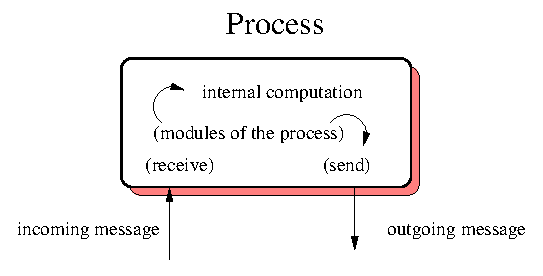
\includegraphics[width=150mm]{figures/step_of_a_process}}
    \caption{Step of a Process \cite[p.~27]{GR06}}
    \label{step_of_a_process}
\end{figure}

\noindent
{\bf Quorum Decisions.}
The problem of atomic consistency is solved by using \emph{quorums}. The first quorum system has been presented in \cite{Gif79} as a technique to maintain the consistency of replicated data. According to \cite{MR97},
\begin{quote}
    A well known way to enhance the availability and performance
    of replicated data is by using \emph{quorums}. A quorum system
    for a universe of servers is a collection of subsets of
    servers, each pair of which intersect. Intuitively, each
    quorum can operate on behalf of the system, thus increasing its
    availability and performance, while the intersection property
    guarantees that operations done on distinct quorums preserve
    consistency.
\end{quote}

From there, the correctness condition for quorum systems follows that if a quorum consists of $n$ processes, at least $(n / 2) + 1$ processes must be available.

In the present model, a quorum decision is defined as either the setting or the measurement of a global clock value. A global clock value exists, if there is a quorum of processes with a common logical clock value, i.e., a majority of processes have synchronous logical clocks.

Since in the system model, each process has a CouchDB instance as part of it, each process has its own logical clock. This is based on the fact that CouchDB's revision numbers are logical timestamps (i.e., they are strictly increasing). Basically, the multiversion concurrency control mechanism constitutes the logical clock, since it assigns the revision numbers; in other words, it provides the clock ticks.

Regarding quorum decisions, the following cases can be differentiated:
\begin{itemize}
    \item When a write operation has committed, a new global clock value was set, i.e., a majority of processes have advanced their logical clocks to the same value.
    \item When a read operation has committed, a global clock value could be measured, i.e., a majority of processes have synchronous logical clocks.
    \item When a data operation has aborted, no assertion can be made about clock synchronicity. Either there is no majority of processes with synchronous logical clocks (if so, the data would be inconsistent), or the data operation has aborted for some other reason (e.g., because the latest revision number was not specified in the write request).
\end{itemize}

\vspace{0.5em}
\noindent
{\bf Eventual Consistency.}
When only eventual consistency is guaranteed, a write request is forwarded by the leader to its assigned CouchDB, and as soon as the according response message has been received, the leader forwards it back to the requesting client. In case that the response message indicates that the write operation has been successful (i.e., it has committed), the written data is eventually replicated to all other base objects.

For read requests, the leader forwards the client's request to its assigned CouchDB, and again, forwards the according response message back to the client as soon it has been received.

For both read and write requests, if a leader has not received any response by its assigned CouchDB within a certain period of time, it sends the client a response with status code {\tt 503 Service Unavailable}.\\

\noindent
{\bf Atomic Consistency.}
In order to guarantee atomic consistency, the leader needs to interact with the other base objects. Each decision made by the leader has to be supported by a quorum of base objects.

When receiving a document read request (i.e.\ a {\tt GET} request), the leader sends a {\tt HEAD} request to the other CouchDBCPs as well as to its assigned CouchDB, in order to retrieve the document revision numbers from the particular CouchDBs. In the response messages, the document revision number is contained in the {\tt ETag} header field. When at least $(n / 2) + 1$ valid response messages (with status code {\tt 200 OK}) have been received, the revision numbers are compared in order to examine whether a quorum for some revision number exists. If that is the case, the leader requests the particular document version from its assigned CouchDB and forwards the response to the requesting client. Otherwise, i.e., if not enough valid response messages have been received, or if there is no quorum for any document version, a response with status code {\tt 503 Service Unavailable} is sent to the client.

When receiving a document write request, the leader forwards it to the other CouchDBCPs as well as to its assigned CouchDB. If at least $n / 2 + 1$ requests succeed, which can be detected by according responses with status code {\tt 201 Created}, one of those responses will be forwarded to the requesting client. Otherwise, a response with status code {\tt 503 Service Unavailable} will be sent.\\

\noindent
{\bf Recovery.}
The system's underlying abstraction for process failure is the crash-recovery abstraction described in \cite[p.~32ff]{GR06}.

A process is faulty if it either crashes and never recovers, or if it keeps crashing and recovering ad infinitum. Otherwise, if the process is always up and running, or if it crashes and recovers a finite number of times, it is correct (i.e., according to this abstraction of a process).

In the crash-recovery abstraction, processes can crash, which means the process stops sending messages, but might later recover. It should be noticed that accordingly, any pattern of message loss (e.g.\ due to network problems) is modeled as a process crash. The difference to an omission fault is that when a process crashes it might lose its internal state.

Figure \ref{failure_modes_of_a_process} depicts the different failure modes; the \emph{arbitrary fault} behavior is the most general one, while the \emph{crash failure}, which means that a process, once it has crashed, does never perform any computation (i.e.\ it does never recover), is the most specific failure mode (c.f.\ \cite[p.~29]{GR06}).

The recovery works as follows. When a write operation commits, the respective leader detects process crashes. If a process crash has been detected, the leader tells all available processes (including itself), to try to notify the crashed process about the missing update. This is what the processes then will do within random periodic time intervals. When the crashed process has eventually recovered, one of its peer processes will finally succeed to notify it about the missing update. Thereupon, the process will send an according read request to its peer processes in order to update the missing document version. Consequently, all peer processes receiving that read request will know that the crashed process has recovered and already been notified about the missing update, and therefore will stop sending any further notifications in this regard. 


\begin{figure}
    \centering
	{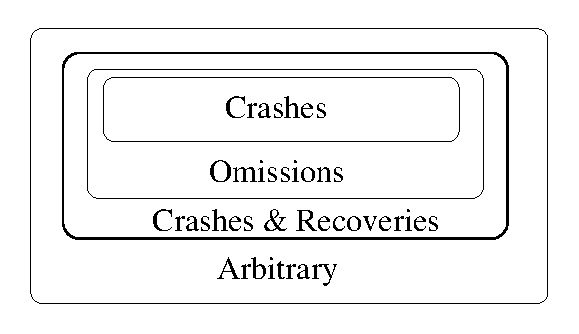
\includegraphics[width=100mm]{figures/failure_modes_of_a_process}}
    \caption{Failure Modes of a Process \cite[p.~30]{GR06}}
    \label{failure_modes_of_a_process}
\end{figure}

\paragraph{System Architecture}
Basically, the system architecture is quite simple. There is a decentralized, client-server style system with redundant CouchDBs, and a CouchDBCP used as a gateway in front of each CouchDB server.

This architecture allows for the achievement of this work's main goal---providing clients with the abstraction of a single reliable CouchDB device, while being able to choose between different consistency guarantees on a per-request basis---by just adding a connector.

The architectural requirements formulated in section \ref{Requirements} are met: there are no single points of failure, and the REST constraints that are kept by CouchDB are not violated.


\section{Correctness}
\noindent
{\bf Atomic Consistency.}
The atomic consistency of a standalone CouchDB instance follows intuitively from multiversion concurrency control (see section \ref{Multiversion Concurrency Control}). Atomic consistency is justified by the very fact that in any write request, clients need to specify the document's current revision number for the write operation to be successful. Therefore, it is impossible that a client overwrites a version whose existence it is not aware of. Moreover, the multiversion concurrency control makes sure that read and write operations are completely isolated from each other, i.e., only committed versions are available for read operations. As a result, all operations on a data object (in the present context a document) are arranged in a total sequential order. This corresponds to the definition of linearizability, which is the correctness condition for concurrently shared atomic data objects.

From the definition of a quorum (see section \ref{System Model}) follows that it is impossible to get more than one different quorum decision at the same point in time. Hence, it is impossible that different clients will succeed in writing different values concurrently, or that different values are returned to different clients' read requests concurrently. As any data operation depends on a quorum decision, this implies that the data operations are totally ordered.

Accordingly, Herlihy and Wing noted that linearizability is a \emph{local} property, which means that it is composable: ``a system is linearizable if each individual object is linearizable. Locality enhances modularity and concurrency, since objects can be implemented and verified independently, and run-time scheduling can be completely decentralized'' \cite{HW87}.\\

\noindent
{\bf Recovery.}
The recovery model is based on the correctness condition for quorum systems, which says that at any time a majority of processes (at least $(n / 2) + 1$) is available, and that base objects eventually recover and cannot be replaced by different processes. In addition, it is assumed that processes recover in the same order they fail, so that the first process that fails is the first one to recover.

As long as these conditions are fulfilled, i.e., if the system behaves correctly, any crashed process, as soon as it has recovered, will eventually be notified about updates it has missed.


\section{Implementation Aspects}

A CouchDBCP prototype has been implemented in Erlang/OTP, using the Mochiweb library as a server connector.

In order to support the cluster-specific semantics, custom header fields are used in the HTTP messages. For example, a CouchDBCP needs to be able to know whether a write request it received was issued by a client or by a CouchDBCP peer. In case the write request was issued by a client, the CouchDBCP would become the leader for that request. In that case, as a leader, it would perform different actions than it would perform as a non-leader.

If a client wants to change the (configurable) default consistency level for a particular request, it sets an accordant field (e.g.\ {\tt X-CouchDBCP-Consistency: atomic}) in the HTTP request header.

A detailed explanation and analysis of the implementation would exceed the scope of this work, and moreover, does not make a lot of sense at this early stage of implementation.

For a small piece of example code from the implementation, see the code listing that is provided in the appendix. The example code is a function that returns the first response from a list of responses to an HTTP {\tt HEAD} request, for whose {\tt ETag} header field value (which is the respective document's revision number) a quorum can be formed. In the case that no quorum can be formed, an error code is returned.


\section{Evaluation}

The prototype that has been developed contains several bugs. Features that are critical in production environments are missing. However, the prototype serves well for demonstration purposes and as a basis for further development. It has been tested being configured for atomic data consistency in a cluster consisting of three base objects; more than half of CouchDB's test cases passed successfully. The goal of developing a prototype that shows that the developed system model forms a valid basis for a practical implementation has been achieved.

The choice to use Erlang/OTP as a programming platform turned out to be a good one. Apparently, Erlang/OTP was designed for such or similar application domains, and hence it can be spoken of as the right tool for that purpose.

In particular, it is Erlang's inherent distributed programming abstractions (most notably processes and asynchronous messaging) that alleviate the development of highly concurrent, fault tolerant distributed programs. To highlight an example, Erlang's processes are extremely cheap with regard to their processing overhead and memory usage. It is possible to have ten-thousandths of processes running in parallel without having a significant decrease on system performance \cite[p.~148ff]{Arm07}.

Erlang discourages the use of shared memory, and mutable data objects in general, but instead encourages the use of high-level programming abstractions, generic design patterns (i.e., OTP \emph{behaviors}, see \cite{LMC10}), and also the use of parallel processes as many as needed, together with asynchronous message passing.

During the prototype implementation, none of Erlang/OTP's approaches revealed any downsides, even though some concepts were new to the author and had to be learned. In fact, the use of Erlang/OTP seems to result in fewer code, faster development, and less bugs, if compared to more mainstream programming platforms, like e.g.\ Java, applied to the same application domain.
